

\begin{figure}[htbp]
    \section*{SMAD2}
\centering
\begin{subfigure}[b]{0.95\textwidth}
\centering
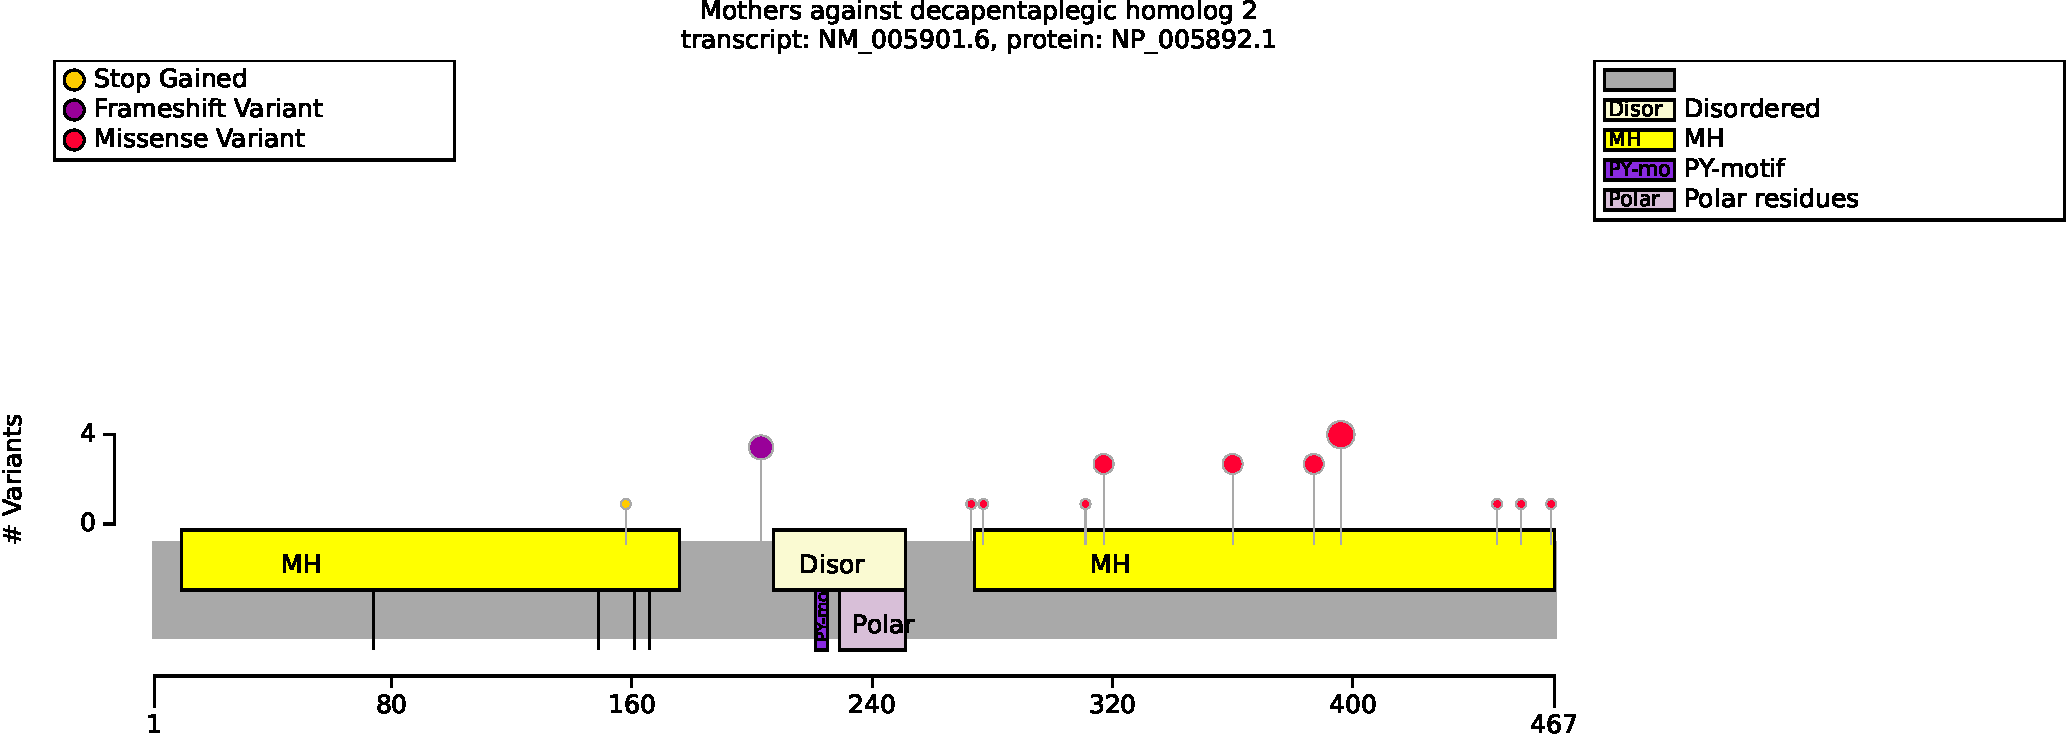
\includegraphics[width=\textwidth]{ img/SMAD2_protein_diagram.pdf} 
\captionsetup{justification=raggedright,singlelinecheck=false}
\caption{Distribution of variants in SMAD2}
\end{subfigure}

\vspace{2em}

\begin{subfigure}[b]{0.95\textwidth}
\centering
\resizebox{\textwidth}{!}{
\begin{tabular}{llllrr}
\toprule
Genotype (A) & Genotype (B) & total tests performed & significant results\\
\midrule
Ser397Tyr & Other & 19 & 0\\
N Term & Other & 19 & 0\\
FEMALE & MALE & 19 & 0\\
\bottomrule
\end{tabular}
}
\captionsetup{justification=raggedright,singlelinecheck=false}
\caption{Fisher Exact Test performed to compare HPO annotation frequency with respect to genotypes.}
\end{subfigure}

\vspace{2em}

\caption{ The cohort comprised 23 individuals (13 females, 8 males, 2 with unknown sex). A total of 89 HPO terms were used to annotate the cohort. Disease diagnoses: Loeys-Dietz syndrome 6 (OMIM:619656) (18 individuals), Congenital heart defects, multiple types, 8, with or without heterotaxy (OMIM:619657) (5 individuals). We were not able to identify published results suggesting correlations with specific SMAD2 residues or variant categories. A total of 23 unique variant alleles were found in \textit{SMAD2} (transcript: \texttt{NM\_005901.6}, protein id: \texttt{NP\_005892.1}).}
\end{figure}
